%\documentstyle[epsf,twocolumn]{jarticle}       %LaTeX2e仕様
\documentclass[twocolumn]{jarticle}     %pLaTeX2e仕様(platex.exeの場合)
%\documentclass[twocolumn]{ujarticle}     %pLaTeX2e仕様(uplatex.exeの場合)
%%%%%%%%%%%%%%%%%%%%%%%%%%%%%%%%%%%%%%%%%%%%%%%%%%%%%%%%%%%%%%
%%
%%  基本バージョン
%%
%%%%%%%%%%%%%%%%%%%%%%%%%%%%%%%%%%%%%%%%%%%%%%%%%%%%%%%%%%%%%%%%
\setlength{\topmargin}{-45pt}
%\setlength{\oddsidemargin}{0cm} 
\setlength{\oddsidemargin}{-7.5mm}
%\setlength{\evensidemargin}{0cm} 
\setlength{\textheight}{24.1cm}
%setlength{\textheight}{25cm} 
\setlength{\textwidth}{17.4cm}
%\setlength{\textwidth}{172mm} 
\setlength{\columnsep}{11mm}

\kanjiskip=.07zw plus.5pt minus.5pt


% 【節が変わるごとに (1.1)(1.2) … (2.1)(2.2) と数式番号をつけるとき】
%\makeatletter
%\renewcommand{\theequation}{%
%\thesection.\arabic{equation}} %\@addtoreset{equation}{section}
%\makeatother

%\renewcommand{\arraystretch}{0.95} 行間の設定

%%%%%%%%%%%%%%%%%%%%%%%%%%%%%%%%%%%%%%%%%%%%%%%%%%%%%%%%
\usepackage[dvipdfmx]{graphicx}   %pLaTeX2e仕様(\documentstyle ->\documentclass)\documentclass[dvipdfmx]{graphicx}
\usepackage[dvipdfmx]{color}
\usepackage[subrefformat=parens]{subcaption}
\usepackage{colortbl}
\usepackage{multicol}
%%%%%%%%%%%%%%%%%%%%%%%%%%%%%%%%%%%%%%%%%%%%%%%%%%%%%%%%

\begin{document}

\twocolumn[
\noindent

\hspace{1em}
\today
\hfill
\ \ 細川 岳大

\vspace{2mm}

\hrule

\begin{center}
{\Large \bf 進捗報告}
\end{center}
\hrule
\vspace{3mm}
]

% ‚ここから 文章 Start!

\section{今週やったこと}
 GAを用いたDataAugmentaion

\section{実験}
前回に引き続きGAを用いたアンサンブル学習のためのDataAugmentationの実験を行った.\\
今回は個体の精度を適応度とした集団1と,後述のfitness2を適応度とした集団2とを,並行して学習を進めた.
共に個体数は15とした.
今回計算量削減のためアンサンブルを行う個体を集団1から上位3つ,集団2から5つを選抜し,集団2ではこの5つの個体を求めて,
精度をよくすることを目標とする.

\subsection{実験データ}
実験データはcifar10を用いて,
事前学習ではepoch数300,train\_dataを各ラベル5000枚の計50000枚使用し,GAで学習する際はepoch数100,train\_dataは各ラベル200枚のオリジナルとそれらすべてをDataAugmentaionしたものとを合わせ計4000枚とし,test\_dataは共に10000枚とした.また事前学習でのaccuracyは0.8475である.
\subsection{遺伝的アルゴリズム}


\subsubsection{探索空間}
\ 探索する水増し操作として画素値操作(Sharpness,Posterize,Brightness,Autoconstrast,Equalize,Solarize,Invert,Contrast,ColorBalance),
変形操作(Mirror,Flip,Translate X/Y,Shear X/Y,Rotate)の16種類の操作であり,今回はそれらすべてを個別にどの程度強くかけるかおよびどの順序でかけるかということを探索する.各操作についての強度の最大最小を設定し,それを-100\%から100\%まで25\%ずつ分11段階の度合いとする.ただし,Autocontrast,Equalize,Invert,Mirror については適用するか否かであるためパラメータが0以上で適用するとした.強度は0から5の整数値を持つ15個の遺伝子を実数値コーディングによって表現する.
また,適用順序に関しては同様に15個の遺伝子を持つ順列コーディングによって表現する.
確率は10\%ごと11段階の実数地コーディングによって表現する.
つまり,探索空間は$2^5*11^{11}*15!*11^{16}$となる.

\subsubsection{選択}
\ 選択について,エリート選出によって最も適応度の高い2つの個体を選択する.なお,この二つは後述する交叉,突然変異は受けずに次の世代に追加する.
残りの選出にはトーナメント選出を用した.トーナメント選出は集団の中から任意の数(トーナメントサイズ)の個体のうち最も適応度の高い個体を選出し次の世代に追加する.今回トーナメントサイズは2とした.
 
\subsubsection{交叉}
\ 強度,確率を表す染色体については2点交叉,順序を表す染色体については部分写像交叉を用いた.2点交叉は一対の親染色体をそれぞれ同じ場所で三分割し中央の染色体を入れ替えて交叉を行う.部分写像交叉は親遺伝子を二分割し入れ替える際重複をなくす交叉法で,重複のあった遺伝子について,それに該当した重複する遺伝子座を見つけ,それに対となっているもう一方の親の遺伝子を参照する.
 
\subsubsection{突然変異}
\ 強度,確率を表す染色体について,対象となる遺伝子の値を各50\%の確率に1増減させ,
 順序を表す染色体について,染色体の一部を逆順にする操作か,染色体を二つに分け前後を入れ替える操作のいずれかを行うものとした.
 
\subsubsection{多様性維持}
\ 多様性を維持するために,上記3つの操作(選択,交叉,突然変異)を行った集団に対し,適用順序を表す染色体について一致するものが3つ以上あれば,
それが2つになるように一部の個体を突然変異させたうえで次の世代の集団とした.
これを集団2にのみ適用した.

\subsubsection{適応度}
\ 集団2において個体$i$のtest\_data10000枚の予測値の集合を${\bf pred}(i)$,accuracyを$f_{acc}({\bf pred}(i))$とし,
予測値の集合の集合$A$に対するアンサンブルによるaccuracyを$f_{ens\_acc}(A)$とする,
また集団1のうち上位3個体の予測値の集合の集合を$B$とする.
\begin{eqnarray*}
	f_{ens\_acc}(X) = f_{acc}\left(\frac{1}{{\rm \#}X}{\displaystyle {\sum_{{\bf a}\in X}{\bf a}}}\right)\\
  	fitness2_{i}
  	= \frac{1}{{}_{15 - 1}\mathrm{C}_{5 - 1}}{\displaystyle {\sum_{A}f_{ens\_acc}(A+B)}}\\
 	U = \{{\bf pred}(1),{\bf pred}(2),...,{\bf pred}( n)\}\\
 	A =  A \subset  U \mid  A\ {\rm have}\ {\bf pred}(i) \land {\rm \#}A=5
\end{eqnarray*}
 とした.
\subsection{実験} 
\subsubsection{パラメータ}
表\ref{tb:param1}に学習パラメータを示す.
\begin{table}[h]
	\centering
	\caption{学習パラメータ\label{tb:param1}}
	\scalebox{1.0}{
		\begin{tabular}{|c||c|} \hline
			optimizer&Adam\\ \hline
			learning rate&0.001\\ \hline
			loss function&categorical\_crossentropy\\ \hline
			batch size&128\\ \hline
			epoch size&30\\ \hline
		\end{tabular}
	}
\end{table}
 表\ref{tb:param_GA}にGAの設定を示す.
\begin{table}[h]
	\centering
	\caption{実験パラメータ\label{tb:param_GA}}
	\scalebox{1.0}{
		\begin{tabular}{|c|c|c|} \hline
			%\multicolumn{2}{|c|}{個体数}&15\\ \hline
			\multicolumn{2}{|c|}{世代数}&32\\ \hline
			\multicolumn{2}{|c|}{交叉率}&0.9\\ \hline\hline
			\multicolumn{3}{|c|}{突然変異率}\\ \hline
			\multicolumn{2}{|c|}{強度,確率(遺伝子ごと)}&0.06\\ \cline{2-3}
			\multicolumn{2}{|c|}{順序(染色体ごと)}&0.1\\ \hline
		\end{tabular}
	}
\end{table}
\subsubsection{結果}
図\ref{fig:graph},にaccuracyの最良値及び平均値の推移を示す.\\

また,今回の最良値が0.8812であり,前回の最良値は0.8846であった.


\subsection{まとめ}
\ 今回の実験で記載はしていないが,集団1よりも集団2のほうが個体ごとのaccuracyが高いものとなっていたが,
個体数や初期値における誤差だと考えられる.しかしその結果,集団2ではaccuracyが高いものほどfitnessも高くなってしまっており,
アンサンブル学習としての意味は少ないように感じた.この結果からアンサンブル学習用の個体を探索するためには先に良個体の探索を済ませたのちに探索したほうが良いと考えられる.また,今まで愚直に平均してfitnessをとっていたが,個体同士の関係をもっとよくみて
fitnessを与えるべきだと思った.


\section{来週の課題}
\begin{itemize}
	\item 前期発表の資料の仕上げ
	\item 絵本についてのリサーチを進める
\end{itemize}

\begin{figure}[b]
	\centering
	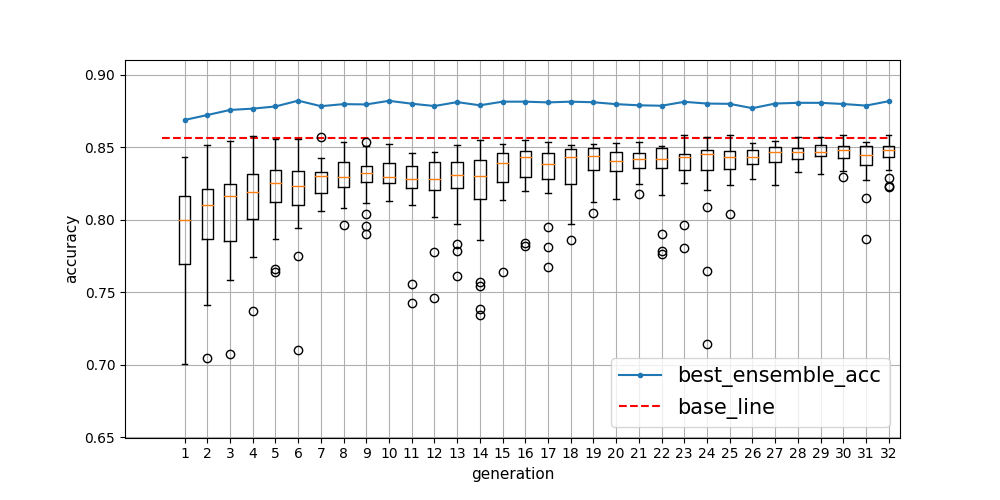
\includegraphics[scale=0.8]{graph.png}
	\caption{集団2のaccuracyの推移\label{fig:graph}}
\end{figure}

\end{document}


